\documentclass{article}
\usepackage[utf8]{inputenc}
\usepackage{anysize}
%\marginsize{2.75cm}{0cm}{4.5cm}{0cm}
\marginsize{0cm}{0cm}{0cm}{0cm}
\usepackage{tikz}
\usetikzlibrary{shapes.geometric, arrows}

\tikzstyle{start} = [ellipse, rounded corners, minimum width=3cm, minimum height=1cm,text centered, draw=black, fill=green!30]
\tikzstyle{stop} = [ellipse, rounded corners, minimum width=3cm, minimum height=1cm,text centered, draw=black, fill=red!30]
\tikzstyle{io} = [trapezium, trapezium left angle=70, trapezium right angle=110, minimum width=1cm, minimum height=1cm, text centered, draw=black, fill=blue!30]
\tikzstyle{process} = [rectangle, minimum width=3cm, minimum height=1cm, text centered, text width=3cm, draw=black, fill=cyan!30]
\tikzstyle{decision} = [diamond, minimum width=3cm, minimum height=1cm, text centered, draw=black, fill=yellow!30]
\tikzstyle{arrow} = [thick,->,>=stealth]

\begin{document}

\thispagestyle{empty}

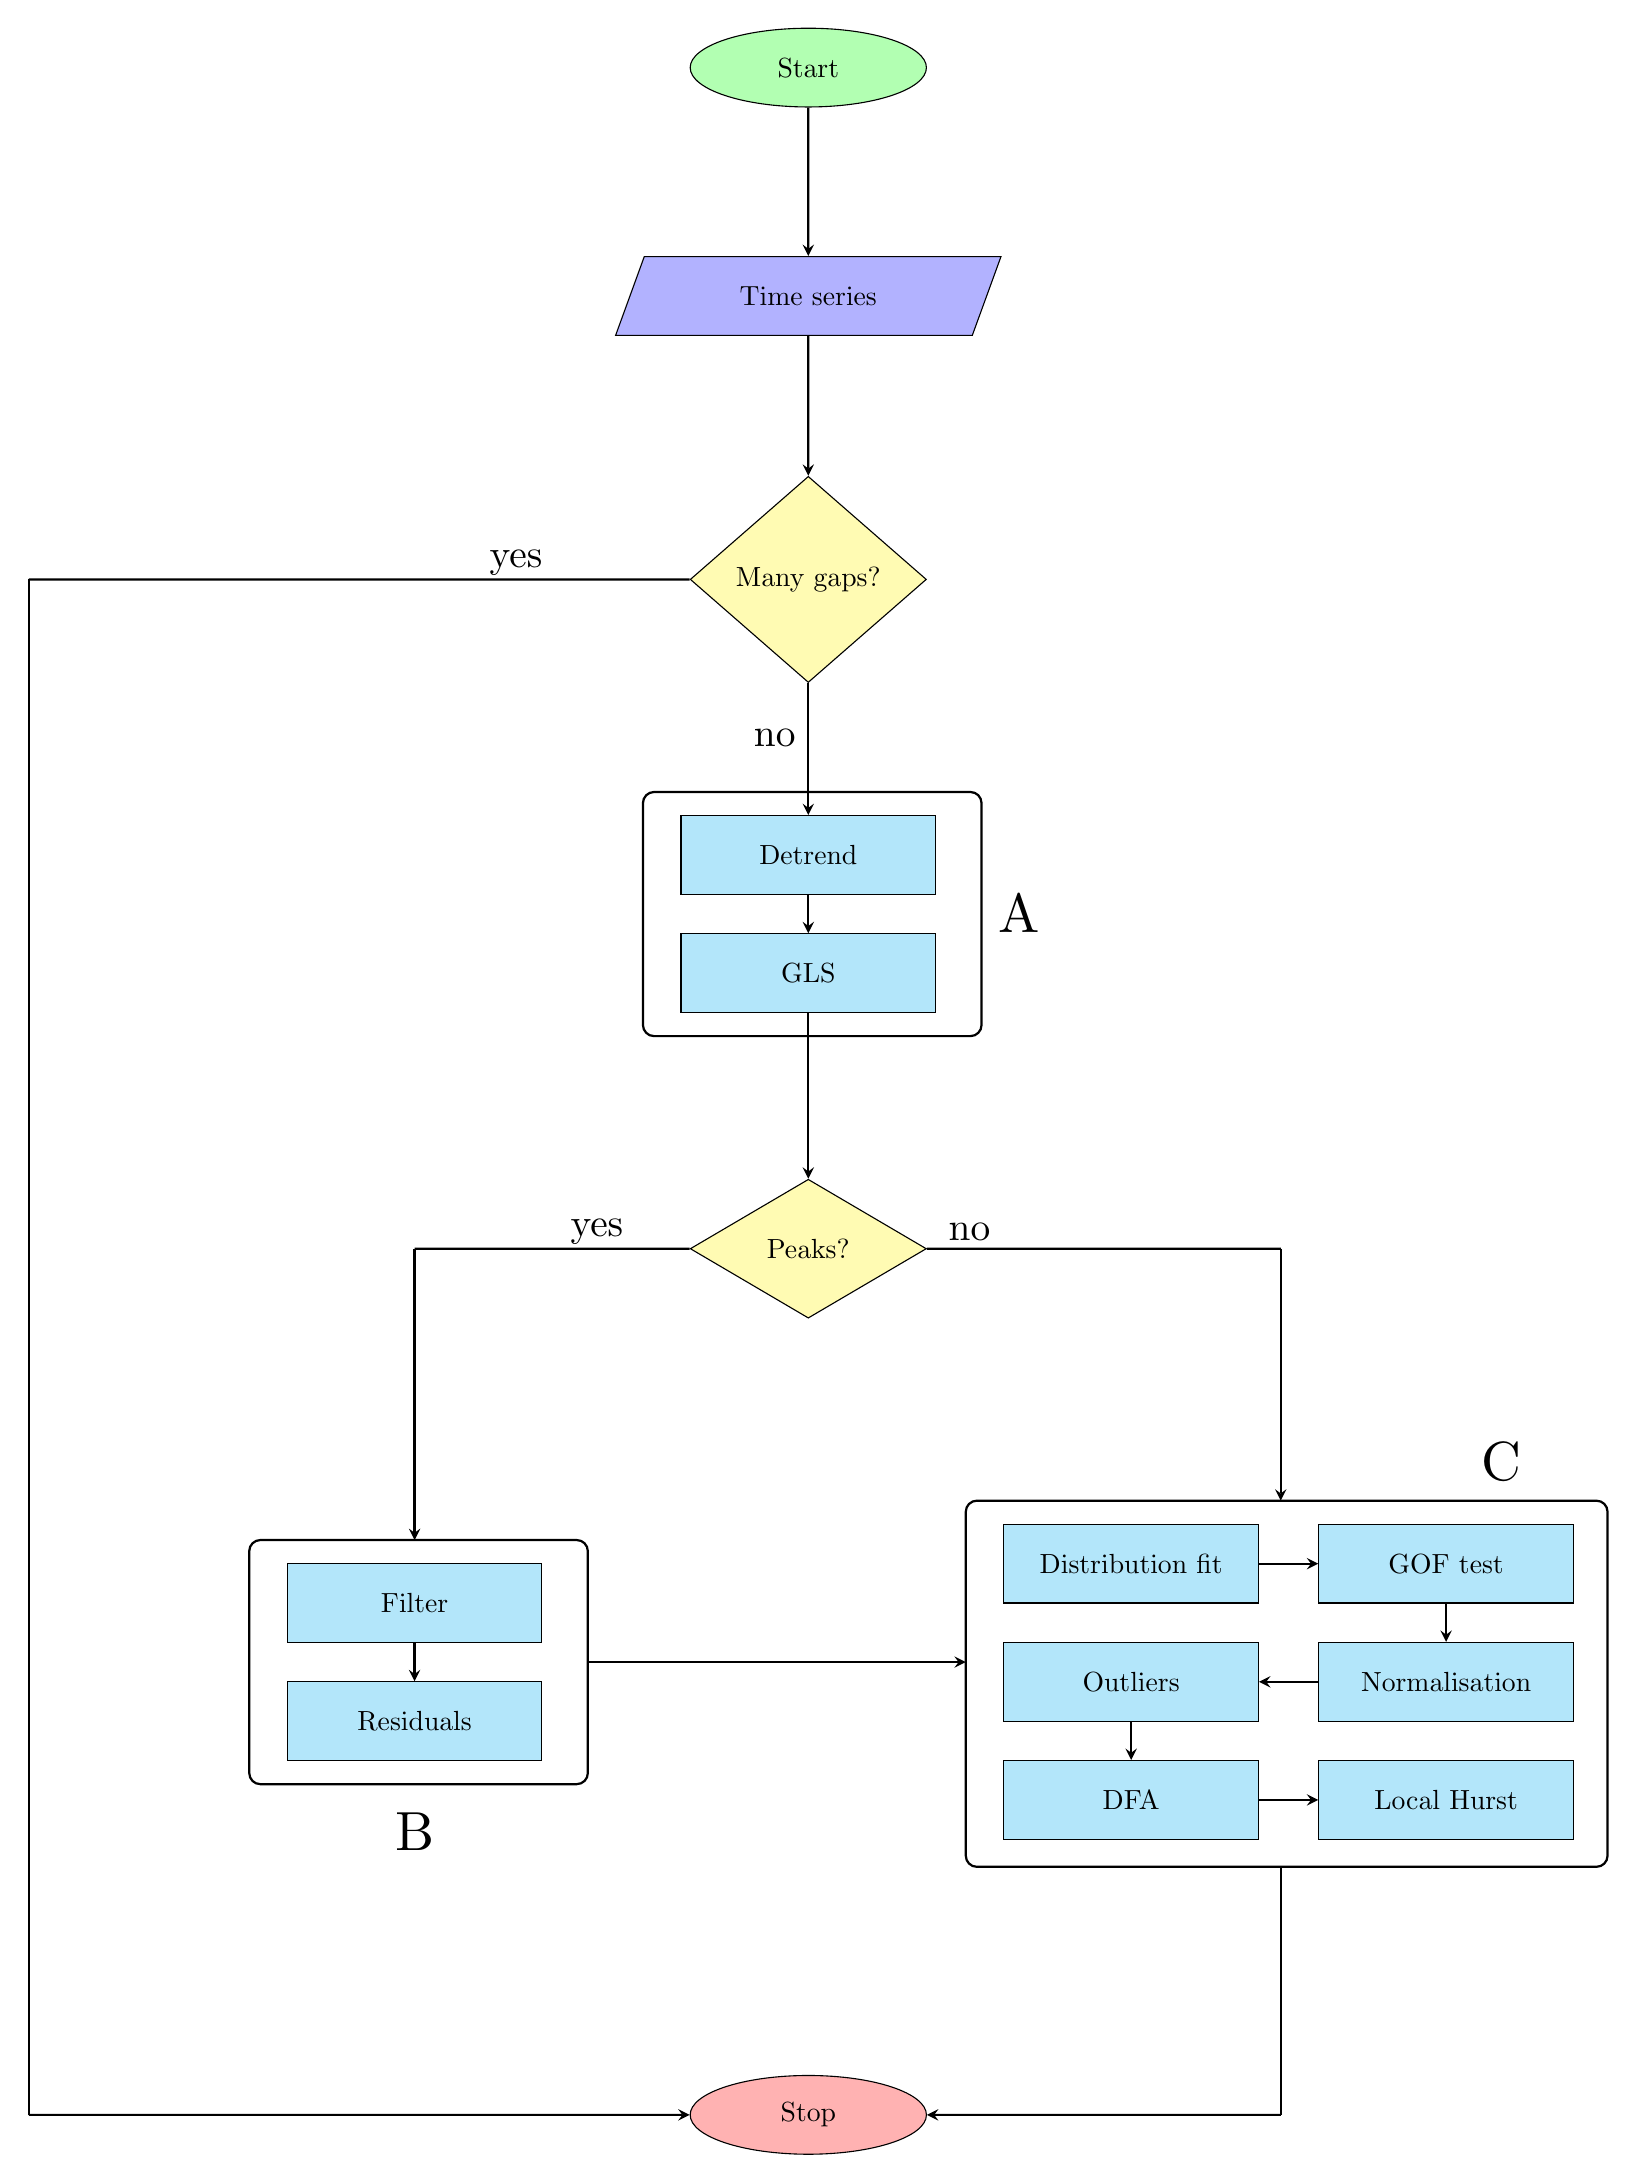
\begin{tikzpicture}%[node distance=2cm]
\centering
\node (start) [start,xshift=2cm,yshift=4cm] {Start};
\node (ts) [io, yshift=1.1cm,xshift=2cm] {Time series};
\node (nan) [decision, yshift=-2.5cm,xshift=2cm] {Many gaps?};
\node (det) [process, yshift=-6cm,xshift=2cm] {Detrend};
\node (gls) [process, yshift=-7.5cm,xshift=2cm] {GLS};
\node (peaks) [decision, yshift=-11cm,xshift=2cm] {Peaks?};
\node (filt) [process, yshift=-15.5cm, xshift=-3cm] {Filter};
\node (res) [process, yshift=-17cm, xshift=-3cm] {Residuals};
\node (dist) [process, yshift=-15cm, xshift=6.1cm] {Distribution fit};
\node (gof) [process, yshift=-15cm, xshift=10.1cm] {GOF test};
\node (out) [process, yshift=-16.5cm, xshift=6.1cm] {Outliers};
\node (norm) [process, yshift=-16.5cm, xshift=10.1cm] {Normalisation};
\node (dfa) [process, yshift=-18cm, xshift=6.1cm] {DFA};
\node (ht) [process, yshift=-18cm, xshift=10.1cm] {Local Hurst};
\node (stop) [stop, yshift=-22cm,xshift=2cm] {Stop};

\draw [thick,rounded corners] (-0.1,-5.2) rectangle ++(4.3,-3.1) node[draw=none,text=black,scale=0.7mm,anchor=east] at (5.2,-6.75) {A};
\draw [thick,rounded corners] (-5.1,-14.7) rectangle ++(4.3,-3.1) node[draw=none,text=black,scale=0.7mm,anchor=south] at (-3,-18.9) {B};
\draw [thick,rounded corners] (4,-14.2) rectangle ++(8.15,-4.65) node[draw=none,text=black,scale=0.7mm,anchor=south] at (10.8,-14.2) {C};

\draw [arrow] (start) -- (ts);
\draw [arrow] (ts) -- (nan);
\draw [arrow] (nan) -- node[scale=0.5mm,yshift=0.1cm,xshift=-0.3cm] {no} (det);
\draw [thick] (nan) -- node[scale=0.5mm,yshift=0.15cm,xshift=1.4cm] {yes} (-7.9,-2.5);
\draw [thick] (-7.9,-2.5) -- (-7.9,-22);
\draw [arrow] (-7.9,-22) -- (stop);
\draw [arrow] (det) -- (gls);
\draw [arrow] (gls) -- (peaks);
\draw [thick] (peaks) -- node[scale=0.5mm,yshift=0.15cm,xshift=-1.2cm] {no} (8,-11);
\draw [arrow] (8,-11) -- (8,-14.2);
\draw [thick] (peaks) -- node[scale=0.5mm,yshift=0.15cm,xshift=0.4cm] {yes} (-3,-11);
\draw [arrow] (-3,-11) -- (-3,-14.7);
\draw [arrow] (-0.8,-16.25) -- (4,-16.25);
\draw [arrow] (filt) -- (res);
\draw [arrow] (dist) -- (gof);
\draw [arrow] (gof) -- (norm);
\draw [arrow] (norm) -- (out);
\draw [arrow] (out) -- (dfa);
\draw [arrow] (dfa) -- (ht);
\draw [thick] (8,-18.85) -- (8,-22);
\draw [arrow] (8,-22) -- (stop);
\end{tikzpicture}

\end{document}